\addchapheadtotoc
\chapter{INTRODUCTION} 
\label{chap:intro}

\section{The problem}
As a student, I've always had a way of \textbf{keeping track of my grades, and making speculations} about what grades I need in upcoming exams to pass my courses. For my own experience, speculating has been a very successful way of focusing my efforts on the right assignments and passing the courses. 

One day, talking to my colleagues, I realized that I wasn't the only student doing this. The reality is that many students chose to aim for the minimum grade instead of performing their best. This may be due to a bunch of reasons, ranging from being lazy to finding the assignments fruitless.

\newpage
\section{The solutions}

\subsection{The expected solution}

The straight forward solution would be that the university provided an official way of seeing the grades of each assignment. But in many cases, it doesn't solve the problem because:
\begin{itemize}[noitemsep]
    \item Some teachers don't publish the grades.
    \item The interface is confusing and difficult to understand.
    \item There's no speculating implemented.
    \item Some universities don't even have this kind of app.
\end{itemize}

Because \textbf{this solution is unreliable}, students that can't benefit from this solution have to come up with their ones.

\subsection{The most used solution}

Each student managed his grades differently. This is the typical procedure I saw students from my faculty following:
\begin{enumerate}
    \item Save the grades in:
    \begin{multicols}{3}
        \begin{itemize}
            \item Notes app
            \item Memory
            \item Agenda
            \item Paper
            \item School portal
            \item Spreadsheet
        \end{itemize}
    \end{multicols}
    \item Speculate the necessary grades. Generally filling the undone exams with made up values, in a test-error way, until getting the desired final grade. Using:
    \begin{multicols}{3}
        \begin{itemize}
            \item Phone basic calculator
            \item Advanced calculator
            \item Spreadsheet
        \end{itemize}
    \end{multicols}
\end{enumerate}

The most used method is writing over, and over, the calculation in the phone calculator until the right value is found. 

In conclusion, \textbf{the whole process is rudimentary and tedious}, it may lead to mistakes in the calculations causing failed courses, and the students not having their grades and speculations easily accessible.

\subsection{The proposed solution}

I suggest making a specific application for this use case. It would be a productivity app that lets students store their grades and also lets them speculate to find the best combination of grades to pass, considering their current ones. All this with excellent ease-of-use.  % The requirements are specified in the \nameref{sec:scope} chapter.

One year ago, I already identified this issue so \textbf{I created a very basic app for myself} that helped me calculating the necessary grades in the upcoming exams to pass my courses. I published it in a domain and shared it with my friends. This started a chain reaction, students started recommending it to their friends because they liked it a lot. Against all odds, the users spread the app through the faculty, to a point that the app had 1,000 views/day during December 2019 (Fig.~\ref{fig:analytics_sessions_1}). Due to this unexpected success, I’d like to improve the app and also make it suitable for other subjects.

As of February 2020, this app doesn't have a database, and subjects are hardcoded by myself, also it is not always working. I developed this project whenever I had free time and I used it as a playground for learning web development. It was a personal project for myself, not thought to be scaled up. The fact that people used it and gave me positive feedback motivated me to improve it. I want to make this app usable by many more students, and let them create and edit subjects, between other things.
% Because of its development methodology and varying skill level, it's gotten messy over time and a lot of things can be improved, but "because they work", I've never spent the time to refactor the entire app, prioritizing adding new functionalities.

% \vfill
% \begin{figure}[h!]
%     \center
%     
\includegraphics[height=12\fontcharht\font`\X]{media/logo-gradecalc.png}
%     \caption{GradeCalc Logo}
% \end{figure}
% \vfill


\vfill
\begin{figure}[h!]
    \center
    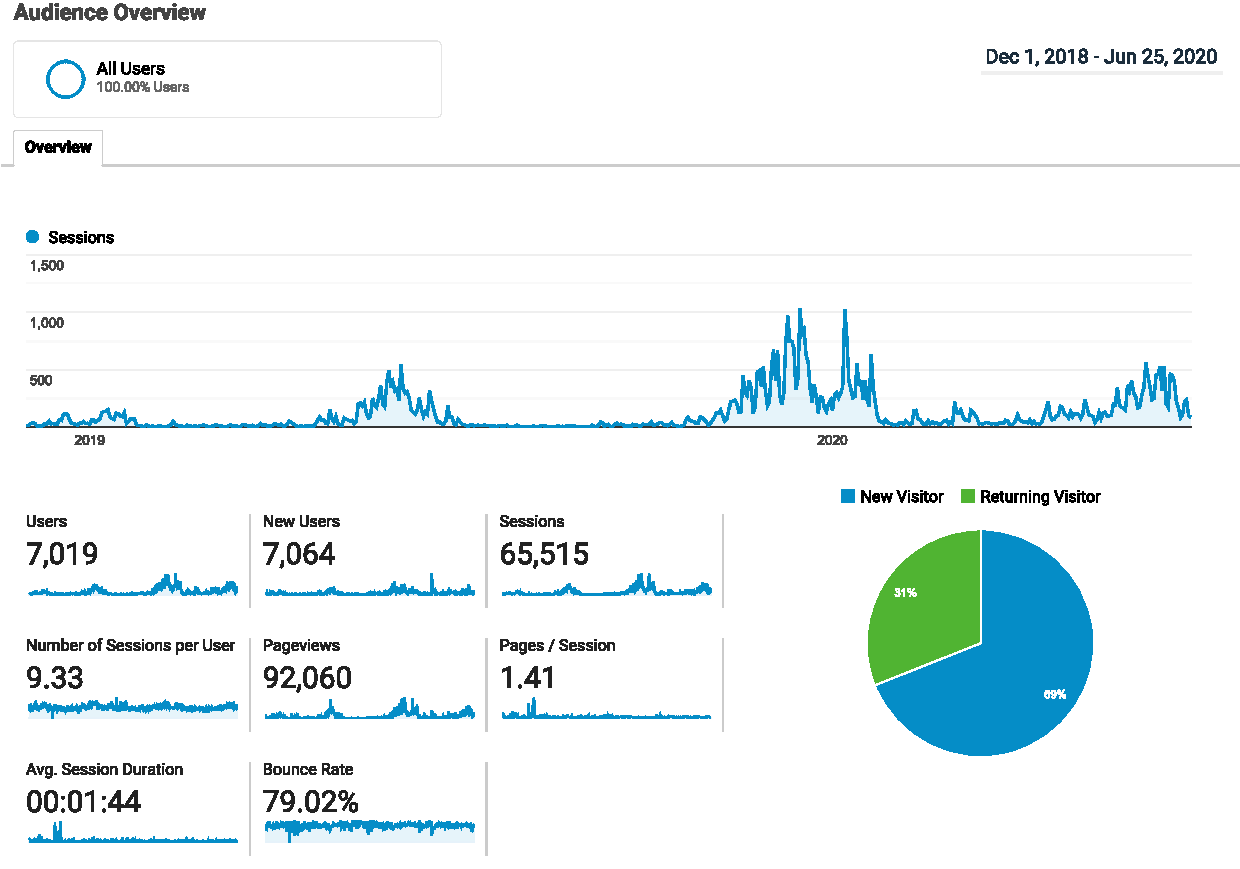
\includegraphics[width=1\columnwidth]{media/analytics.pdf}
    \caption{GradeCalc analytics - Sessions from Dec 2018 to June 2020}
    \label{fig:analytics_sessions_1}
\end{figure}
\vfill

% \section{The new app}

% I plan to improve the app following best practices. To the eyes of the user this new app it should look like a visual and performance update with added features. On the other hand, to the eyes of the developer, it will look like a completely different app with very little code reused. The most reused things will be user experience design.

% The new app will use a Javascript framework, so the majority of UI interaction code will need to be updated or discarded. Besides, my skill level when I started developing the app has drastically increased and. So a lot of code will be discarded.

% Summarizing, this project will be about making a renewed app with the same or more features from the old one but improving it's scalability, maintainability, robustness, and code quality in general. The most changes will be under the hood, in a seamless manner for the current users.

\clearpage\newpage
\section{State of the Art}

\subsection{Generic grade calculators}
There are plenty of generic grade calculators, but they don't fulfill the needs of UPC students because they lack the following key features:
\begin{itemize}
    \setlength\itemsep{-0.5em}
    \item Can't save grades nor evaluation formulas.
    \item Doesn't estimate the necessary grade to pass.
    \item You have to rewrite all the parameters every time you refresh.
    \item They have a very bad user experience.
    \item Most of them use the American F-A system instead of the Spanish 0-10 system.
\end{itemize}
In fact, using the phone calculator is faster than this kind of apps.

\begin{figure}[ht!]
    \centering
\begin{subfigure}{0.3\textwidth}
  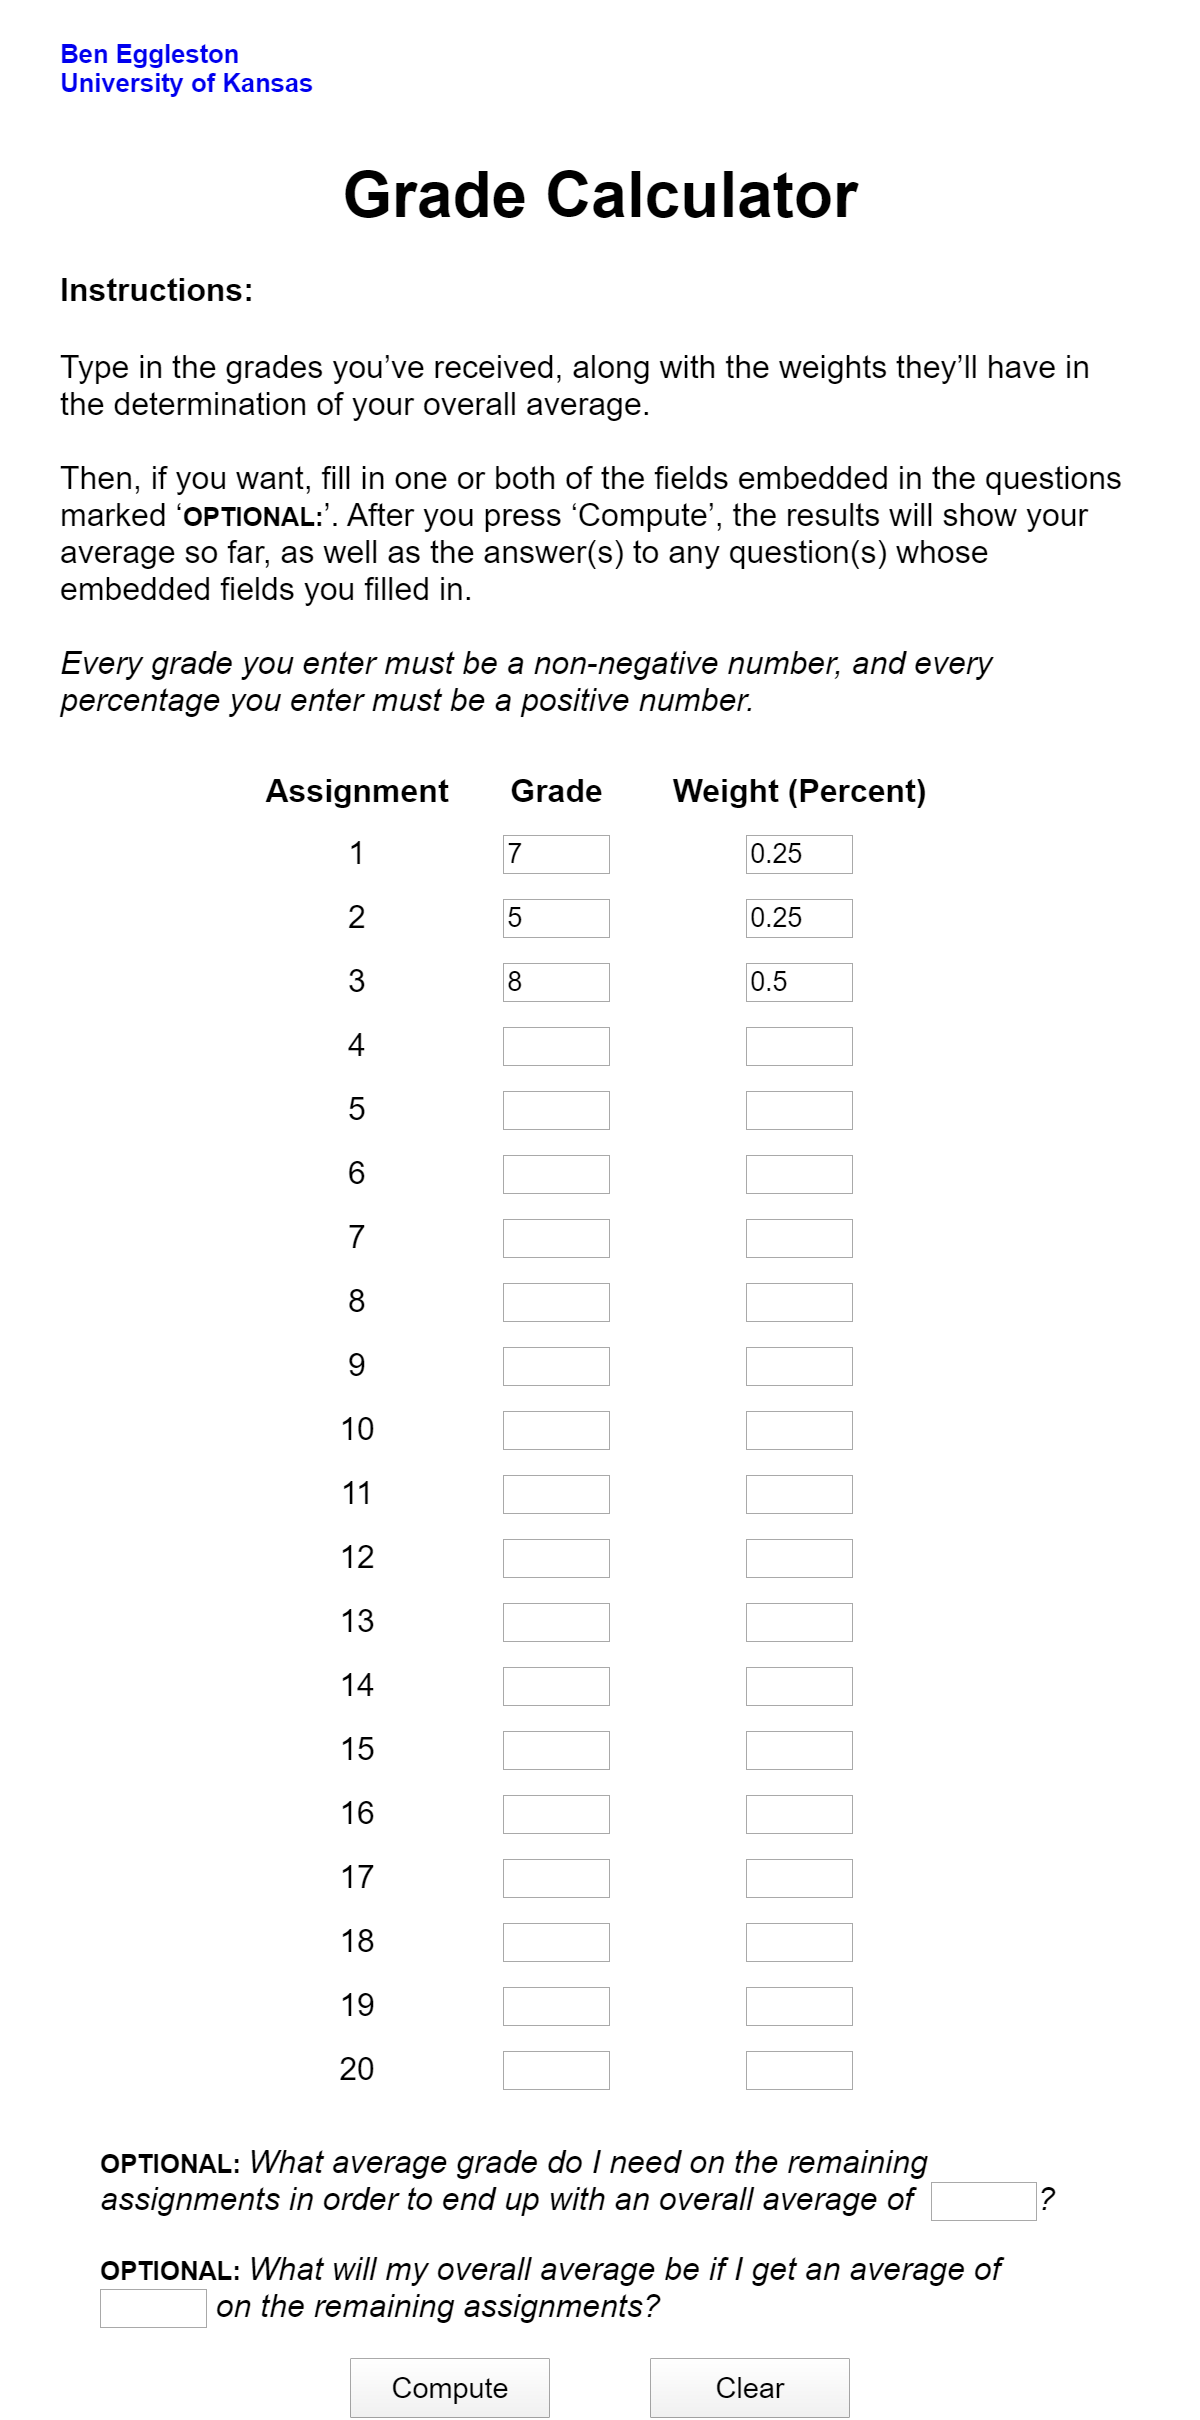
\includegraphics[frame,width=\linewidth]{media/grade-calculator-ben.png}
    \caption[Ben Eggleston]{Ben Eggleston \cite{grade-calculator-ben}}
    \label{grade-calculator-ben}
\end{subfigure}\hfil
\begin{subfigure}{0.3\textwidth}
  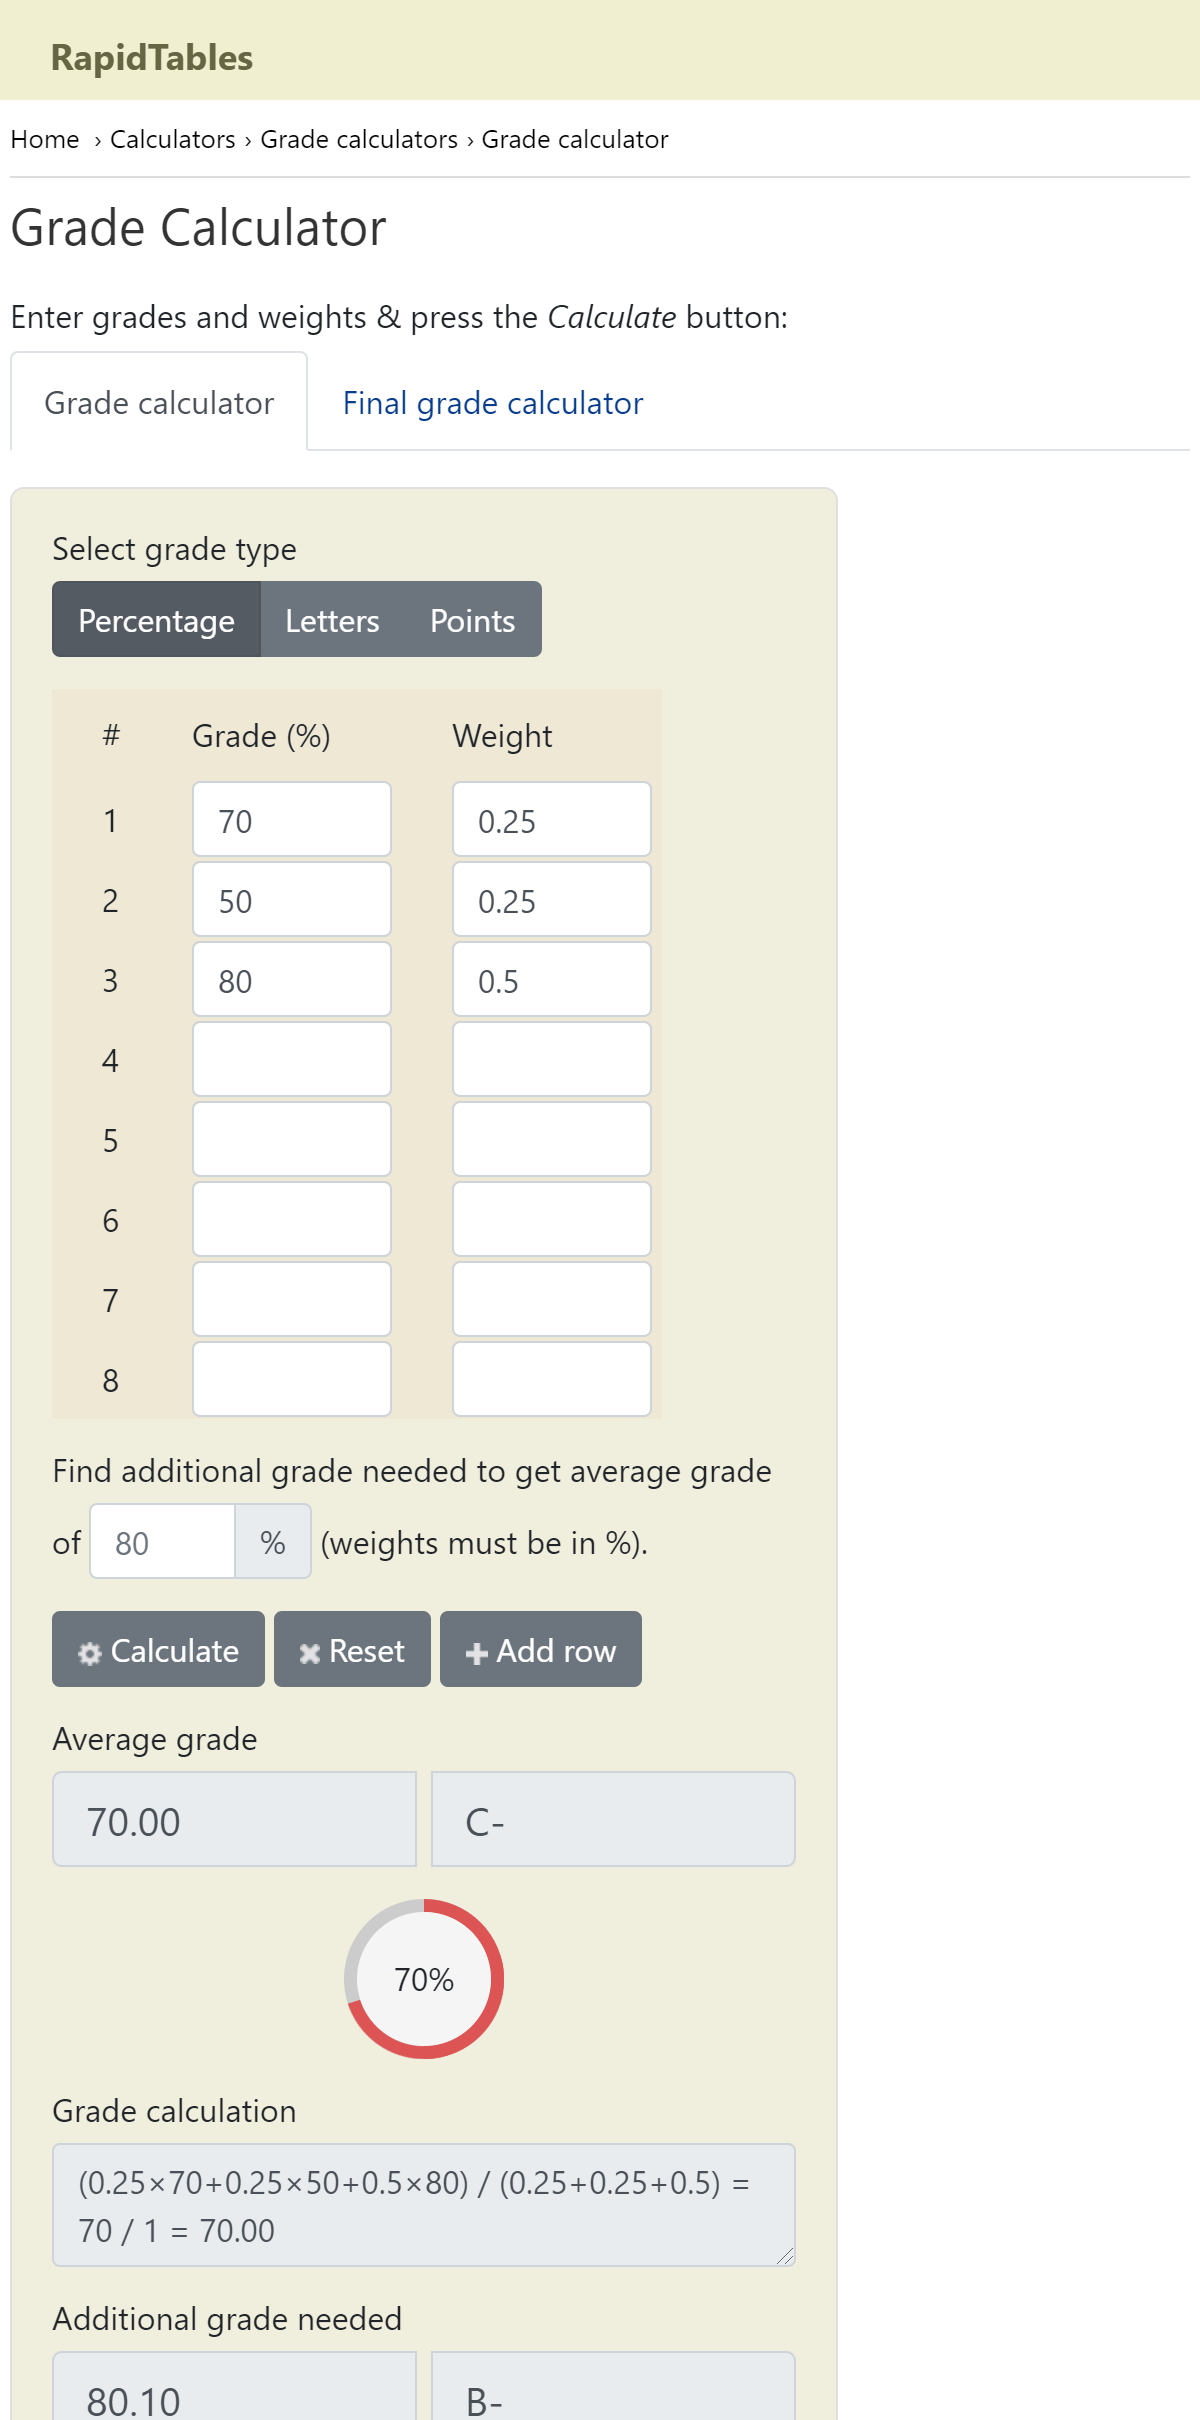
\includegraphics[frame,width=\linewidth]{media/grade-calculator-rapid.png}
\caption[RapidTables]{RapidTables \cite{grade-calculator-rapid}}
\label{grade-calculator-rapid}
\end{subfigure}
\caption{Generic grade calculators}
\label{fig:images}
\end{figure}

\subsection{Atenea - UPC's virtual campus}
UPC University has an online campus platform that includes a qualification table, where students can see their current grade.
\begin{itemize}
    \setlength\itemsep{-0.5em}
    \item Not available for all courses.
    \item Not available outside UPC.
    \item Doesn't estimate the necessary grade to pass.
\end{itemize}

\begin{figure}[h!]
    \center
    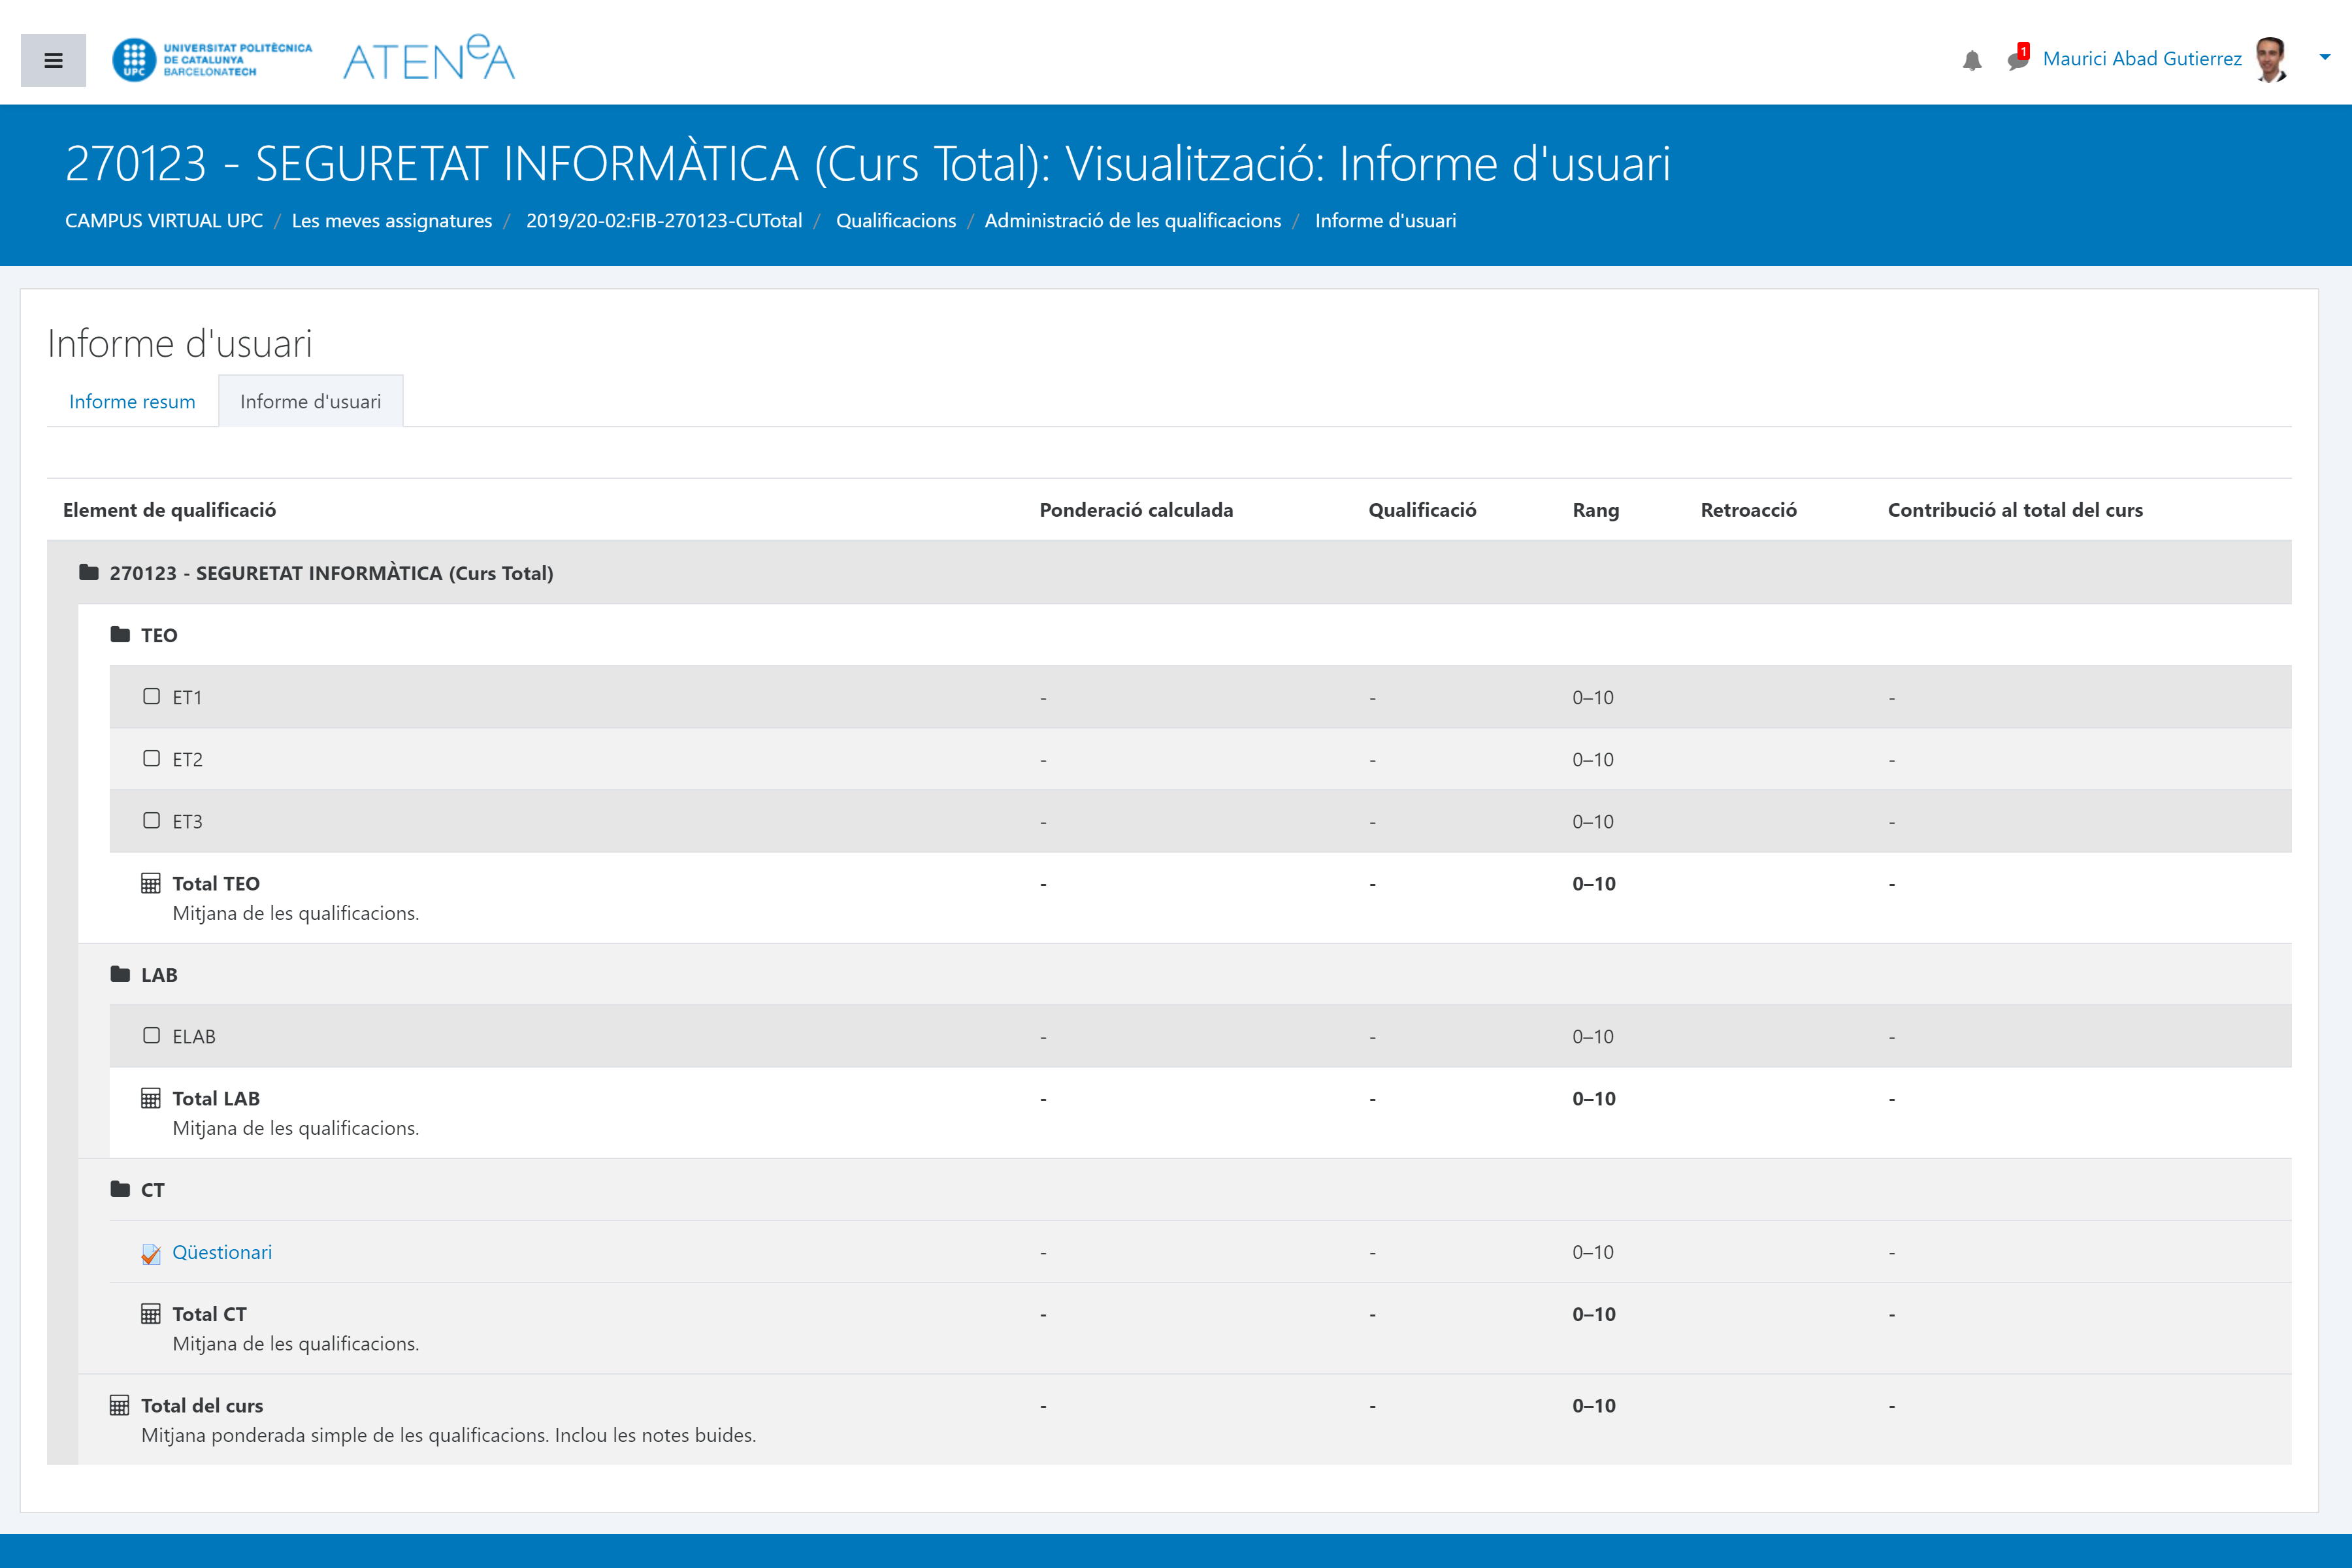
\includegraphics[frame,width=.8\columnwidth]{media/atenea.png}
    \caption[Atenea UPC]{Atenea UPC \cite{atenea}}
    \label{atenea}
\end{figure}

\subsection{Spreadsheet document}
Some students use a spreadsheet to calculate their grades, but it has many disadvantages:
\begin{itemize}
    \setlength\itemsep{-0.5em}
    \item Not accessible from the phone.
    \item You have to enter all evaluation formulas.
    \item Not specific to the use case.
    \item Doesn't estimate the necessary grade to pass.
\end{itemize}

\newpage
\section{Stakeholders}
The main users are going to be Students of Informatics Engineering in UPC, so they are the most important stakeholder. Then there are students on the same campus, and then from all Barcelona faculties.

Another really important stakeholders are the Developers from the community, that are going to voluntarily help in the development of the app, they need to be satisfied to keep developing or the app won't be able to get updates.

Finally, there are the users who use the app. They must be really satisfied to share the app with their friends if the app becomes popular it will help more students.

\begin{figure}[ht!]
    \centercenter
    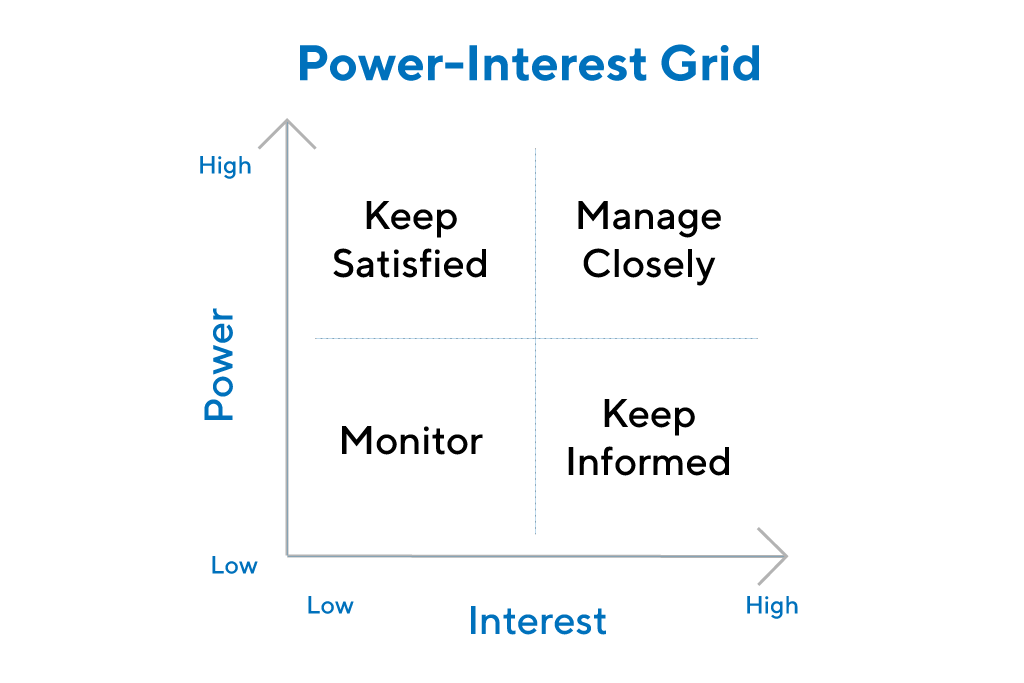
\includegraphics[width=1\columnwidth]{media/power-interest-grid.png}
    \caption[Power-Interest grid]{Power-Interest grid \cite{stakeholder-analysis}}
    \label{power-interest_grid}
\end{figure}

\pagebreak
\begin{framed}
\begin{multicols}{4}
\noindent
\tikzcircle[fill=Green]{6pt} Manage Closely

\noindent
\tikzcircle[fill=Cyan]{6pt} Keep Satisfied

\noindent
\tikzcircle[fill=Goldenrod]{6pt} Keep Informed

\noindent
\tikzcircle[fill=Magenta]{6pt} Monitor
\end{multicols}
\end{framed}

\noindent
This is the stakeholder list with its Power-Interest category:
\begin{itemize}
    \item \tikzcircle[fill=Green]{6pt} Developers
    \item \tikzcircle[fill=Magenta]{6pt} UPC University
    \item \tikzcircle[fill=Green]{6pt} Students
    \begin{itemize}
        \item By degree:
        \begin{itemize}
            \item \tikzcircle[fill=Green]{6pt} \textbf{Students of Informatics Engineering in UPC}
            \item \tikzcircle[fill=Green]{6pt} Students of Telecommunications Engineering in UPC
            \item \tikzcircle[fill=Cyan]{6pt} Students of other degrees
        \end{itemize}
        \item By location:
        \begin{itemize}
            \item \tikzcircle[fill=Green]{6pt} Students in Barcelona
            \item \tikzcircle[fill=Goldenrod]{6pt} Students in Spain
            \item \tikzcircle[fill=Magenta]{6pt} Students from everywhere
        \end{itemize}
        \item By app experience:
        \begin{itemize}
            \item \tikzcircle[fill=Green]{6pt} Students that are enjoying the app
            \item \tikzcircle[fill=Green]{6pt} Students that know and use the app
            \item \tikzcircle[fill=Magenta]{6pt} Students that don't know the app
        \end{itemize}
    \end{itemize}
\end{itemize}
